\section{函数的极限}
\label{sec:ru-function-limits}
\label{sec:analysis-function-limits}

数列的下标按自然数逐项增加，函数的输入却可以从许多实数位置靠近同一点。例如$(x^2-1)/(x-1)$在$x=1$没有定义，但$x\neq1$时它等于$x+1$，邻近输入的输出仍趋于$2$。
函数极限研究的正是这种去掉中心点后的共同趋近，不要求函数在中心有取值。本节先给出定义和几种变形，再借数列极限建立存在性判别和运算法则，最后求出指数函数与三角函数在原点附近的基本极限。

\subsection{函数极限的定义、无穷小与无穷大}
\label{sec:ru-function-limit-definition}

讨论$x$靠近$a$，要先说清哪些点算靠近。以$a$为中心、半径为$r$的开区间$(a-r,a+r)$称为$a$的一个邻域，去掉中心后的$(a-r,a)\cup(a,a+r)$称为去心邻域。

还须保证定义域中确实有不同于$a$的点能够任意靠近$a$。设$X\subseteq\mathbb R$，若$a$的每个去心邻域都含有$X$中的点，就称$a$为$X$的\term{聚点}（cluster point）；
$a$本身可以不属于$X$，例如$0$是$(0,1)$的聚点。$X$中不是聚点的点称为\term{孤立点}（isolated point），例如整数集合中的每个点：附近没有其他输入，谈不上趋近。

\begin{definition}[函数的极限]
\label{def:ru-function-limit}
设$f:X\to\mathbb R$，$a$为$X$的聚点，$b\in\mathbb R$。若对每个$\varepsilon>0$，都存在$\delta>0$，使
\[
 x\in X,\quad0<|x-a|<\delta\quad\Longrightarrow\quad|f(x)-b|<\varepsilon,
\]
就称$x\to a$时$f(x)$的极限为$b$，记作$\lim_{x\to a}f(x)=b$或$f(x)\to b$（$x\to a$）。
\end{definition}
这里用输入误差$\delta$控制输出误差$\varepsilon$，与数列用尾部起点控制误差的思路相同。条件$0<|x-a|$排除了中心点，所以既不要求$f(a)$有定义，也不要求它等于$b$。
回到开头的例子：$x\neq1$时$f(x)=x+1$，给定$\varepsilon>0$取$\delta=\varepsilon$，则$0<|x-1|<\delta$时$|f(x)-2|=|x-1|<\varepsilon$，所以极限为$2$。

图~\ref{fig:analysis-process-epsilon-delta-band}把输入邻域与输出误差带对应起来，并把中心处的函数值与极限分开。

\begin{figure}[!htbp]
 \centering
 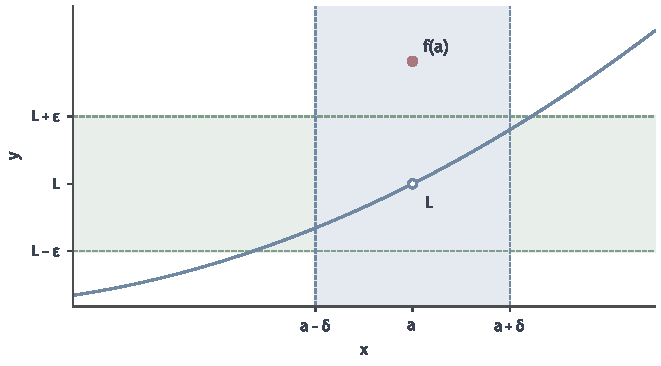
\includegraphics[width=112.0mm]{figures/01-mathematical-preliminaries-upper/00-shared/matplotlib/chapter3-concept-processes/epsilon-delta-band.pdf}
 \caption{取$a=L=1$（$L$即正文中的极限值$b$），$x\neq1$时$f(x)=x^2$，另令$f(1)=2$。蓝带对应$\delta=0.2$的输入范围，绿带对应$\varepsilon=0.55$的输出范围；去掉$a$后，蓝带内曲线全部落在绿带内。空心点是极限位置，红实心点是$f(a)$，不参加去心邻域条件。}
 \label{fig:analysis-process-epsilon-delta-band}
\end{figure}

\paragraph{单侧极限与无穷处的极限}
实轴上的输入可以从两侧接近一点，两侧的输出未必有相同趋向。只让$x<a$的输入趋近$a$，得到左极限$\lim_{x\to a^-}f(x)$；只让$x>a$的输入趋近，得到右极限$\lim_{x\to a^+}f(x)$。
两者分别在上述条件中加上$x<a$或$x>a$，并要求那一侧有定义域中的点任意靠近$a$。两侧都能趋近时，极限存在当且仅当左右极限都存在且相等。

例如阶跃函数$\mathbb I\{x\geq0\}$在$0$处的左极限为$0$、右极限为$1$，所以极限不存在。在闭区间$[a,b]$上，左端点只能从右侧趋近，右端点只能从左侧趋近，端点处的极限总是指单侧极限。

输入还可以趋向无穷。设定义域向右无界，$\lim_{x\to+\infty}f(x)=b$表示：对每个$\varepsilon>0$，存在$M$使定义域中所有$x>M$都满足$|f(x)-b|<\varepsilon$；$x\to-\infty$类似。

输出也可以越过任何有限界：对有限聚点$a$，$f(x)\to+\infty$（$x\to a$）表示对每个实数$M$都存在$\delta>0$，使定义域中满足$0<|x-a|<\delta$的$x$都有$f(x)>M$。
以$1/x$为例：$x\to\pm\infty$时它趋于$0$，这是输入趋向无穷；$x\to0^+$时它趋于$+\infty$，$x\to0^-$时趋于$-\infty$，这是输出趋向无穷，两侧方向不同，因而没有共同的双侧极限。

\paragraph{无穷小、无穷大与渐近记号}
\label{sec:comb-growth-scales}
趋向零的量出现在误差、余项和微分中，需要一个统一的名称。在指定的趋向下极限为$0$的函数或数列称为\term{无穷小}（infinitesimal），绝对值趋于$+\infty$的称为无穷大。

例如$x\to0$时$x$与$x^2$都是无穷小，$n\to\infty$时$1/n$是无穷小。无穷小描述的是一个变化过程的极限性质，不是某个固定的很小的数。若$f$在趋向附近非零，则$f$为无穷大当且仅当$1/f$为无穷小。

两个无穷小趋于零的相对速度可以不同，比较它们的比值即可。设在所讨论的趋向附近$g\neq0$。
\begin{definition}[渐近记号]
\label{def:ru-asymptotic-notation}
若$f/g\to0$，记$f=o(g)$，表示$f$相对于$g$可以忽略；若$|f/g|$在趋向附近有界，即存在常数$C$使最终$|f|\leq C|g|$，记$f=O(g)$；若$f/g\to1$，记$f\sim g$，称二者等价。
\end{definition}
例如$x\to0$时$x^2=o(x)$，$3x=O(x)$但不是$o(x)$，$x+x^2\sim x$。比值把这些记号与相对误差联系起来：$f\sim g$恰好说明用$g$近似$f$的相对误差$|f-g|/|g|$趋于零。

等价无穷小可以在乘除中互相替换：若$f\sim f_1$、$g\sim g_1$，则$fg/(f_1g_1)=(f/f_1)(g/g_1)\to1$。相减时却不行，因为主要部分可能相互抵消。
例如$x\to0$时$f(x)=x+x^2$与$g(x)=x$都等价于$x$，若把两者都换成$x$再相减会得到$0$，而实际上$f-g=x^2$。抵消以后，留下的是原先被忽略的高阶部分，必须保留更精细的展开才能判断。

同样的记号可用于$n\to\infty$的数列，用来比较增长的快慢。$3n+7=O(n)$、$n/10=O(n)$，但两个比值分别趋于$3$和$0.1$，都不是$o(n)$；$10\sqrt n=o(n)$，因为$10\sqrt n/n\to0$。

对最终为正的数列，若存在$c>0$使$a_n\geq cb_n$最终成立，记$a_n=\Omega(b_n)$；同时满足$O$与$\Omega$时记$a_n=\Theta(b_n)$，表示同一数量级。
$n=O(n^2)$也成立，所以大$O$只给出上界，不一定是精确的增长阶。后文描述算法的计算量时沿用这里的含义，比较的始终是两个数量的比值。
图~\ref{fig:vol1-add-asymptotic-ratios}画出了上面三个比值。

\begin{figure}[!htb]
 \centering
 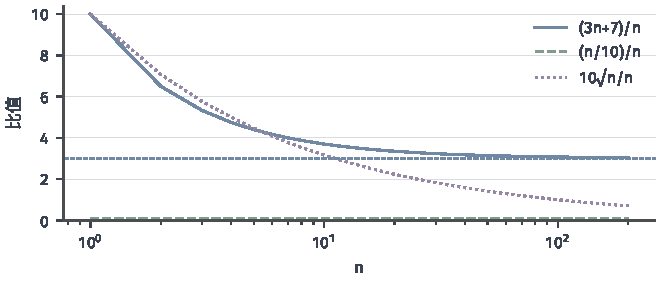
\includegraphics[width=112mm]{figures/01-mathematical-preliminaries-upper/00-shared/matplotlib/mathematical-language-combinatorics-analysis-optimization-comprehension-additions/asymptotic-ratios.pdf}
 \caption{三个解析数列除以$n$后的比值，展示整数$n=1,\ldots,200$，横轴为对数刻度。蓝、绿、紫线的极限分别为$3,0.1,0$。前两者对应$O(n)$而非$o(n)$，第三者对应$o(n)$；极限由正文中的表达式判断，有限范围曲线只帮助观察。}
 \label{fig:vol1-add-asymptotic-ratios}
\end{figure}

\subsection{函数极限存在的判别}
\label{sec:ru-function-limit-criteria}

函数极限要求控制$a$附近所有允许的输入，直接验证并不方便。下面的序列判据把它转化为数列极限，使上一节的工具可以直接使用。
\begin{theorem}[函数极限的序列判据]
\label{thm:ru-sequential-criterion}
设$a$为$X$的聚点。$\lim_{x\to a}f(x)=b$，当且仅当对每个满足$x_n\in X\setminus\{a\}$且$x_n\to a$的数列，都有$f(x_n)\to b$。
\end{theorem}
\begin{proof}
设函数极限为$b$。给定$\varepsilon$取相应的$\delta$，充分靠后的$x_n$满足$0<|x_n-a|<\delta$，于是$|f(x_n)-b|<\varepsilon$。

反过来用反证法。若误差条件不成立，就存在$\varepsilon_0>0$，使每个$\delta=1/n$都不合要求，即可选$x_n\in X$满足$0<|x_n-a|<1/n$而$|f(x_n)-b|\geq\varepsilon_0$；这列输入趋于$a$，输出却不趋于$b$。
\end{proof}
序列判据也是否定极限存在的常用工具：只要找到两列趋于$a$的输入，使输出趋于不同的值。例如$f(x)=\sin(1/x)$，沿$x_n=1/(2n\pi+\pi/2)$恒有$f(x_n)=1$，沿$y_n=1/(2n\pi+3\pi/2)$恒有$f(y_n)=-1$，所以$x\to0$时极限不存在。

不知道候选极限时，也可以像数列那样检查输出是否彼此接近。
\begin{theorem}[函数极限的柯西准则]
\label{thm:ru-function-cauchy}
设$a$为$X$的聚点。$x\to a$时$f(x)$有有限极限，当且仅当对每个$\varepsilon>0$，都存在$\delta>0$，使任意两个满足$0<|x-a|<\delta$、$0<|y-a|<\delta$的$x,y\in X$都有$|f(x)-f(y)|<\varepsilon$。
\end{theorem}
\begin{proof}
必要性由三角不等式得到：两个输出都与极限相差不到$\varepsilon/2$。

充分性先固定一列$x_n\in X\setminus\{a\}$、$x_n\to a$。对给定的$\varepsilon$，充分靠后的$x_n,x_m$都落在$\delta$去心邻域内，所以$(f(x_n))$是柯西数列，由实数的完备性收敛到某个$b$。
另取一列$y_n\to a$，把两列交错排成$x_1,y_1,x_2,y_2,\ldots$，它仍趋于$a$，输出列同样收敛；它的两个子列$(f(x_n))$与$(f(y_n))$必有同一极限。
所以每列趋于$a$的输入都给出同一个$b$，由序列判据，$f(x)\to b$。
\end{proof}
准则中的两个输入都不等于$a$，这与极限只看去心邻域的约定一致。数列的柯西准则依赖确界原理，这里通过它同样依赖实数的完备性。

\paragraph{极限的运算法则}
借助序列判据，数列极限的运算法则可以逐条搬到函数上。
\begin{theorem}[函数极限的运算法则]
\label{thm:ru-function-limit-laws}
设$a$为$X$的聚点，$f,g:X\to\mathbb R$，$x\to a$时$f(x)\to b$、$g(x)\to c$，其中$b,c\in\mathbb R$，$\lambda$为实常数，则$x\to a$时
\begin{enumerate}
 \item 和与差：$f(x)\pm g(x)\to b\pm c$；
 \item 数乘：$\lambda f(x)\to\lambda b$；
 \item 积：$f(x)g(x)\to bc$；
 \item 商：若$c\neq0$，则在$a$的某个去心邻域内$g\neq0$，并且$f(x)/g(x)\to b/c$。
\end{enumerate}
\end{theorem}
\begin{proof}
任取$x_n\in X\setminus\{a\}$、$x_n\to a$，由序列判据，$f(x_n)\to b$、$g(x_n)\to c$。对这两列数分别使用定理~\ref{thm:ru-sequence-limit-laws}中的和、差、数乘与积的法则，再由序列判据返回函数极限，即得前三条。

对商，先在$g$的极限定义中取$\varepsilon=|c|/2$，得到一个去心邻域，其中$|g(x)|>|c|/2>0$；在这个邻域内任取趋于$a$的输入列，用数列的商法则，再由序列判据返回。
\end{proof}
分子分母都趋于零时不能套用商的法则。例如$(x^2-1)/(x-1)$在$x\to1$时须先约去公因子$x-1$，才能求出极限$2$。

\begin{theorem}[函数极限的夹逼定理]
\label{thm:ru-function-squeeze}
若在$a$的某个去心邻域内，所有允许的输入都满足$u(x)\leq h(x)\leq v(x)$，且$x\to a$时$u(x)\to L$、$v(x)\to L$，其中$L\in\mathbb R$，则$h(x)\to L$。
\end{theorem}
\begin{proof}
任给$\varepsilon>0$，取一个共同的去心邻域，使其中$u(x)$与$v(x)$都落在$(L-\varepsilon,L+\varepsilon)$内，夹在中间的$h(x)$也在其中。
\end{proof}
例如$-|x|\leq x\sin(1/x)\leq|x|$，所以$x\to0$时$x\sin(1/x)\to0$。

复合函数的极限需要多一点小心。设$x\to a$时$f(x)\to b$，$y\to b$时$g(y)\to c$。若在$a$的某个去心邻域内$f(x)\neq b$，或者$g$在$b$处有定义且$g(b)=c$，则$g(f(x))\to c$。

没有这两个条件之一，结论可能失败：令$f\equiv b$为常数，$g(y)=1$（$y\neq b$）、$g(b)=0$，则$y\to b$时$g(y)\to1$，但$g(f(x))\equiv0$。
问题在于外层的极限只看$b$的去心邻域，而内层的输出可能恰好落在被排除的$b$上；第一个条件保证这种情形不发生，第二个条件则说明即使发生也没有影响。

\subsection{基本函数的极限}
\label{sec:ru-elementary-limits}

上一章把指数和三角函数当作已知对象。现在有了级数和函数极限，可以给出指数函数的定义，并求出后面计算导数要用的两个基本极限。

\paragraph{自然指数函数}
对每个实数$x$，级数$\sum_{k\geq0}x^k/k!$相邻项绝对值之比为$|x|/(k+1)\to0$，由比值判别绝对收敛。定义
\[
 \exp x=\sum_{k=0}^\infty\frac{x^k}{k!}.
\]

指数函数最重要的性质是加法公式$\exp(x+y)=\exp x\,\exp y$。证明要计算两个级数的乘积，先说明绝对收敛级数可以按总次数归并。

设$\sum_ka_k$与$\sum_jb_j$绝对收敛。有限的正方形和满足$\sum_{k,j\leq N}a_kb_j=(\sum_{k\leq N}a_k)(\sum_{j\leq N}b_j)$，因此趋于两个和的乘积。
按总次数$k+j=n\leq N$归并的三角形和，与正方形和只差满足$k,j\leq N$、$k+j>N$的项；这些项中$k$或$j$大于$N/2$，其绝对值之和不超过
$(\sum_{k>N/2}|a_k|)(\sum_j|b_j|)+(\sum_k|a_k|)(\sum_{j>N/2}|b_j|)$，它随$N$增大趋于零。所以按总次数归并后得到同一极限。

用于指数级数，第$n$组为$\sum_{k=0}^nx^ky^{n-k}/[k!(n-k)!]$，由二项式定理它等于$(x+y)^n/n!$，于是
\[
 \exp x\,\exp y=\sum_{n=0}^\infty\frac{(x+y)^n}{n!}=\exp(x+y).
\]
记$e=\exp1\approx2.71828$。由加法公式，对正整数$n$有$\exp n=e^n$，因此通常把$\exp x$写作$e^x$。

加法公式推出了上一章当作已知的几条性质。由$e^xe^{-x}=e^0=1$知$e^x\neq0$，又$e^x=(e^{x/2})^2\geq0$，所以$e^x>0$。
对$u\geq0$，级数各项非负，只保留前两项便得$e^u\geq1+u$；于是$h>0$时$e^{x+h}=e^xe^h\geq e^x(1+h)>e^x$，指数函数严格递增。
同一不等式说明$x\to+\infty$时$e^x\to+\infty$，再由$e^x=1/e^{-x}$得$x\to-\infty$时$e^x\to0$。

原点附近的变化可以直接从级数估计。当$0<|h|<1/2$时，由$1/k!\leq1$，
\[
 |e^h-1-h|\leq\sum_{k=2}^\infty|h|^k=\frac{h^2}{1-|h|}\leq2h^2.
\]
除以$|h|$得$|(e^h-1)/h-1|\leq2|h|$，因此
\[
 \lim_{h\to0}\frac{e^h-1}{h}=1.
\]
这一推导只用到级数的估计，没有用到导数或逐项求导。同一估计还给出$|e^{x+h}-e^x|=e^x|e^h-1|\leq e^x(|h|+2h^2)\to0$，下一节将据此说明指数函数连续，并构造它的反函数自然对数。

\paragraph{三角函数的基本极限}
三角函数的基本极限来自单位圆上的几何比较。设$0<h<\pi/2$，比较单位圆中以$h$为圆心角的内接三角形、扇形与外切三角形的面积，得到$\sin h\leq h\leq\tan h$，即
\[
 \cos h\leq\frac{\sin h}h\leq1.
\]
又由$1-\cos h=2\sin^2(h/2)\leq h^2/2$，得到$0\leq1-\sin h/h\leq h^2/2$。$\sin h/h$是偶函数，同一估计对$h<0$也成立，由夹逼定理，
\[
 \lim_{h\to0}\frac{\sin h}h=1,\qquad\lim_{h\to0}\frac{\cos h-1}h=0,
\]
后者来自$|1-\cos h|/|h|\leq|h|/2$。第一个极限恰为$1$，依赖于用弧长度量角；若用角度制，会多出比例系数$\pi/180$。
